\section{Auswertung}
\label{sec:Auswertung}
\subsection{Bestimmung des RC-Glieds}
Die Messung wird wie in der Duchtführung beschrieben durchgeführt.
Die so erhaltenen Messwerte befinden sich in Tabelle\ref{tab:Messwerte1} :
\begin{table}[H]
    \centering
    \caption{Kondensatorspannung bei fester Frequenz.}
    \label{tab:Messwerte1}
    \begin{tabular}{S[table-format=1.1] S[table-format=2.2] }
        \toprule
        {$t/\si{\milli\second}$} & {$U_C/\si{\volt}$} \\
        \midrule
        0.2 & 14.00 \\
        0.4 & 11.10 \\
        0.6 & 8.64  \\
        0.8 & 6.72  \\
        1.0 & 5.36  \\
        1.2 & 4.08  \\
        1.4 & 3.20  \\
        1.6 & 2.48  \\
        1.8 & 1.92  \\
        2.0 & 1.60  \\
        2.2 & 1.28  \\
        2.4 & 0.96  \\

        \bottomrule
    \end{tabular}
\end{table}

\noindent Die Messwerte werden in der halblogarithmischen Abbildung aufgetragen.
Es wird eine lineare Ausgleichsrechnung, mit Python, durchgeführt und aufgetragen.
Diese hat eine Steigung von $m=\SI{-1.03\pm0.14}{\per\milli\second}$
und einen $y$-Achsenabschnitt von $b=(2.75\pm0.19)$.

\begin{figure}
    \centering
    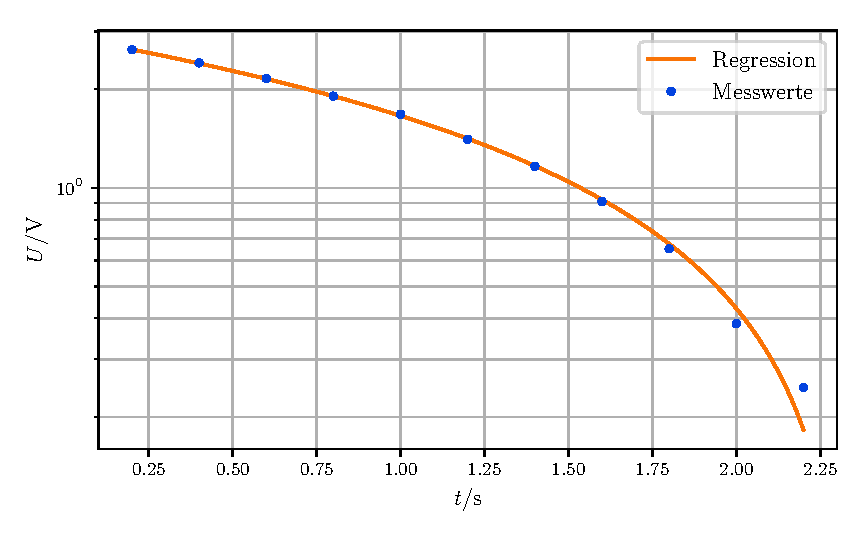
\includegraphics{build/messung1.pdf}
    \caption{Messwerte und Ausgleichsgerade.}
    \label{fig:plot1}
\end{figure}

Die Steigung ist hier $\frac{1}{RC}$ .
Damit ist $RC$ der Kehrwert der Steigung.
\begin{equation*}
  RC=\SI{0.97\pm0.14}{\milli\second}
\end{equation*}
\subsection{Frequenzabhängigkeit der Kondensatorspannung}
Die Messung wird wie in der Durchführung beschrieben ausgeführt.
Die so erhaltenen Messwerte befinden sich in Tabelle\ref{tab:Messwerte2}:
\begin{table}[H]
    \centering
    \caption{Kondensatorspannung bei variabler Frequenz.}
    \label{tab:Messwerte2}
    \begin{tabular}{S[table-format=6.2] S[table-format=2.3] }
        \toprule
        {$f/\si{\hertz}$} & {$U_C/\si{\volt}$} \\
        \midrule
        10.00 & 12.670\\
        12.08 & 12.670\\
        14.94 & 12.750\\
        17.96 & 12.830\\
        20.01 & 12.830\\
        30.00 & 12.860\\
        50.00 & 12.510\\
        80.50 & 11.960\\
        100.00 & 11.480\\
        200.36 & 9.110\\
        300.00  & 7.290\\
        500.00 &  4.790\\
        799.36 &  3.170\\
        1000.00 & 2.530\\
        2000.00 & 1.290\\
        3004.00 & 0.879\\
        3500.00 & 0.768\\
        5000.00 & 0.522\\
        8000.00 & 0.327\\
        10000.00 &  0.263\\
        20000.00 &  0.131\\
        50000.00 &  0.053\\

        \bottomrule
    \end{tabular}
\end{table}
\noindent Die Werte werden in Abbildung aufgetragen.
Durch diese wird eine nichtlineare Ausgleichskurve,mit Gleichung\eqref{eq:gl4}, gezogen.
\begin{figure}
    \centering
    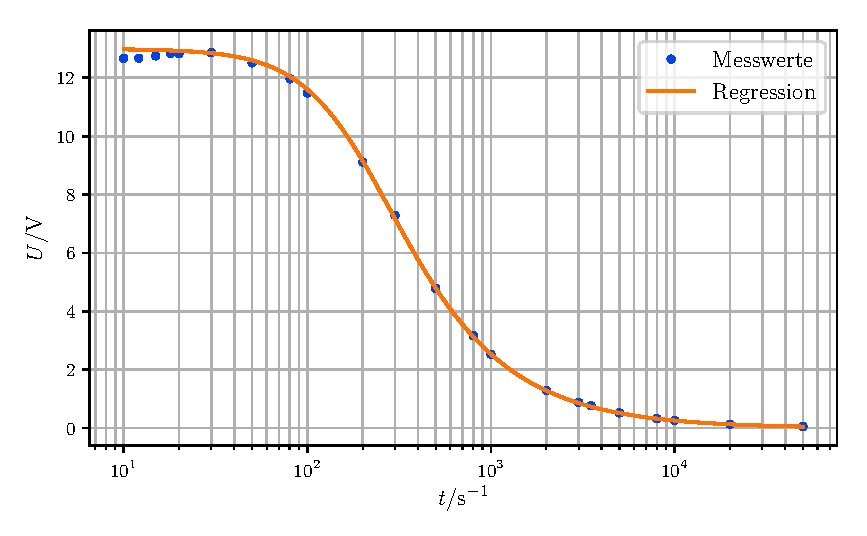
\includegraphics{build/messung2.pdf}
    \caption{Messwerte.}
    \label{fig:plot2}
\end{figure}
